% Created 2024-05-20 Mon 01:41
% Intended LaTeX compiler: lualatex
\documentclass[bigger]{beamer}
\usepackage{amsmath}
\usepackage{fontspec}
\usepackage{graphicx}
\usepackage{longtable}
\usepackage{wrapfig}
\usepackage{rotating}
\usepackage[normalem]{ulem}
\usepackage{capt-of}
\usepackage{hyperref}
\usetheme[progressbar=foot, sectionpage=none, numbering=fraction]{metropolis}
\usepackage{tikz}
\usepackage{booktabs}
\usepackage{adjustbox}
\usepackage{diagbox}
\usepackage{latexcolors}
\usetikzlibrary{automata, positioning, arrows, arrows.meta}
\usepackage{diagbox}
\usepackage{dsfont}
\usepackage{amsmath}
\usepackage{fontawesome}
\usepackage{pgfgantt}
\usepackage[ruled]{algorithm2e}
\usepackage[absolute, overlay]{textpos}
\definecolor{RedBrown}{RGB}{192, 4, 4} \setbeamercolor{progress bar}{fg=RedBrown} \setbeamercolor{title separator}{fg=RedBrown}
\setbeamercolor{progress bar in head/foot}{fg=RedBrown} \setbeamercolor{progress bar in section page}{fg=RedBrown} \setbeamercolor{alerted text}{fg=RedBrown}
\pretocmd{\tableofcontents}{\thispagestyle{empty}}{}{}
\addtocounter{framenumber}{-1}
\usepackage{listings}
\usepackage{xcolor}
\definecolor{codegreen}{rgb}{0,0.6,0}
\definecolor{codegray}{rgb}{0.5,0.5,0.5}
\definecolor{codepurple}{rgb}{0.58,0,0.82}
\definecolor{backcolour}{HTML}{f0f0f0}
\lstdefinestyle{mystyle}{
backgroundcolor=\color{backcolour},
commentstyle=\color{codegreen},
keywordstyle=\color{magenta},
numberstyle=\tiny\color{codegray},
stringstyle=\color{codepurple},
basicstyle=\ttfamily,
breakatwhitespace=false,
breaklines=true,
captionpos=b,
keepspaces=true,
numbers=none,
numbersep=5pt,
showspaces=false,
showstringspaces=false,
showtabs=false,
tabsize=2
}
\lstset{style=mystyle}
\usetheme{default}
\author{Andrea Pierré}
\date{May 20, 2024}
\title{Research plan}
\subtitle{Lab meeting}
\institute{Brown University}
\titlegraphic{\hfill
\includegraphics[height=1.5cm]{img/Brown Logo_2016_2 Color Process ST_1300.png}}
\setbeamercovered{transparent=10}
\setbeamertemplate{section in toc}[sections numbered]
\AtBeginSection[]{\begin{frame}[plain, noframenumbering]{Outline}    \setbeamertemplate{section in toc}[sections numbered]\setbeamertemplate{subsection in toc}[subsections numbered]\tableofcontents[currentsection, currentsubsection]\end{frame}}
\AtBeginSubsection[]{\begin{frame}[plain, noframenumbering]{Outline}\setbeamertemplate{section in toc}[sections numbered]\setbeamertemplate{subsection in toc}[subsections numbered]\tableofcontents[currentsection,currentsubsection]\end{frame}}
\hypersetup{
 pdfauthor={Andrea Pierré},
 pdftitle={Research plan},
 pdfkeywords={},
 pdfsubject={},
 pdfcreator={Emacs 29.3 (Org mode 9.7)}, 
 pdflang={English}}
\begin{document}

\maketitle
\begin{frame}[plain]{Outline}
\tableofcontents
\end{frame}

\section{Context \faicon{question-circle}}
\label{sec:orgd5c51ff}

\begin{frame}[<+->][label={sec:org61b5b9c}]{Why modeling?}
\begin{itemize}
\item Posit: You understand a system if you can simulate it
\end{itemize}
\begin{quote}
What I cannot create, I do not understand. --Richard Feynman
\end{quote}
\begin{itemize}
\item If you have a good enough model you may uncover mechanisms that explain a phenomena
\begin{itemize}
\item Without a model \(\to\) you're limited to describe the \alert{how}
\item With a model \(\to\) you may be able to explain the \alert{why}
\end{itemize}
\item Test hypothesis
\item Abstraction of the system: makes you think of the parameters/inputs/outputs
\item Find out what is needed to reproduce experimental results, what explains those results
\end{itemize}
\end{frame}
\begin{frame}[<+->][label={sec:org2708416}]{What do we want to know?}
\begin{itemize}
\item Understand what the network learns
\(\to\) What \alert{function} does it learns?
\item How the constrains of the task affect learning \& the representations learned?
\item Does the network learn something related to the real neurons? (million \faicon{dollar}\faicon{dollar}\faicon{dollar} question)
\end{itemize}
\end{frame}
\begin{frame}[<+->][label={sec:org5f26c38}]{Compositional hypothesis}
\begin{itemize}
\item Does the network learn a generalizable policy? \(\to\)~How to test it?
\begin{itemize}
\item From indexed locations (current) to coordinate system
\item Merged actions space
\end{itemize}
\end{itemize}
\end{frame}
\begin{frame}[label={sec:org046f332}]{Compositional hypothesis}
\begin{center}
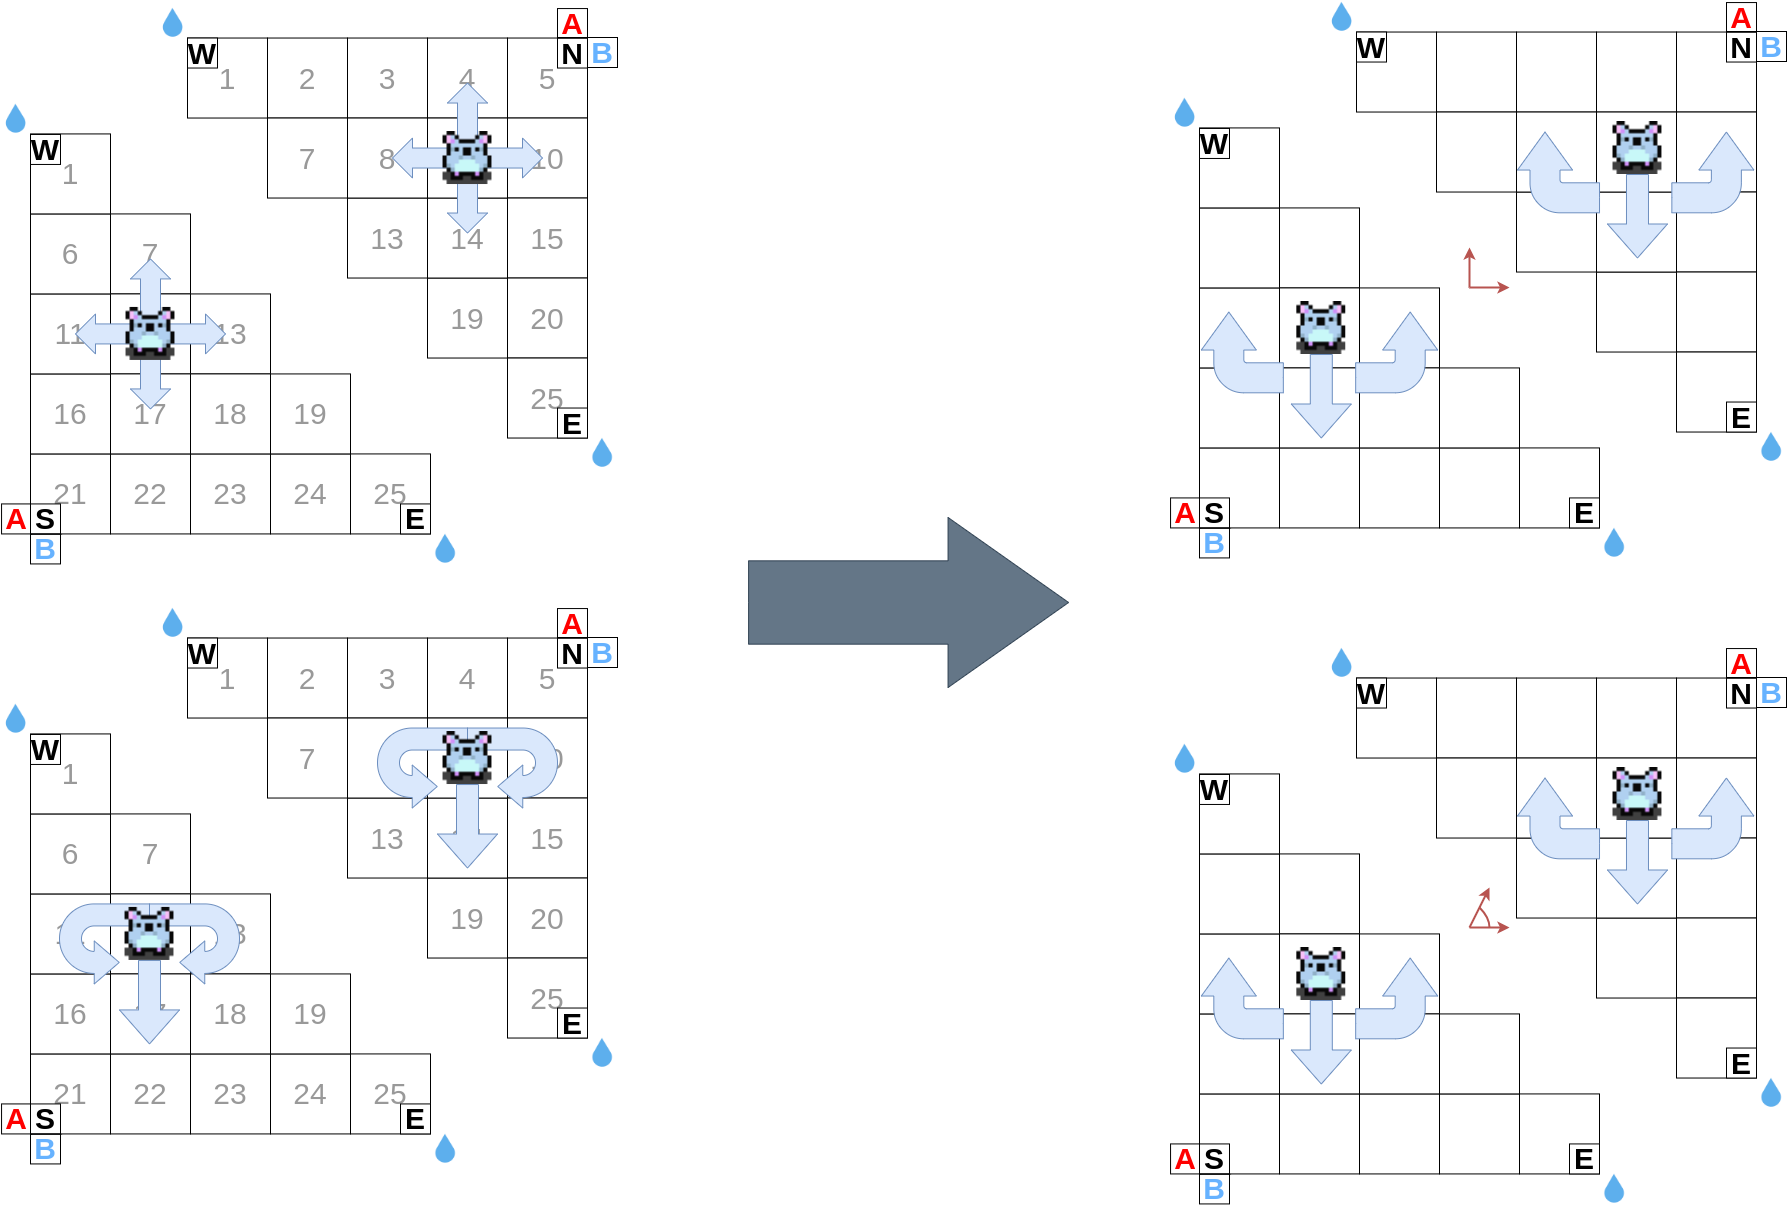
\includegraphics[width=.9\linewidth]{img/env_new-triangle-task.drawio.png}
\end{center}
\end{frame}
\begin{frame}[label={sec:orga3d528c}]{Implementation}
\begin{center}
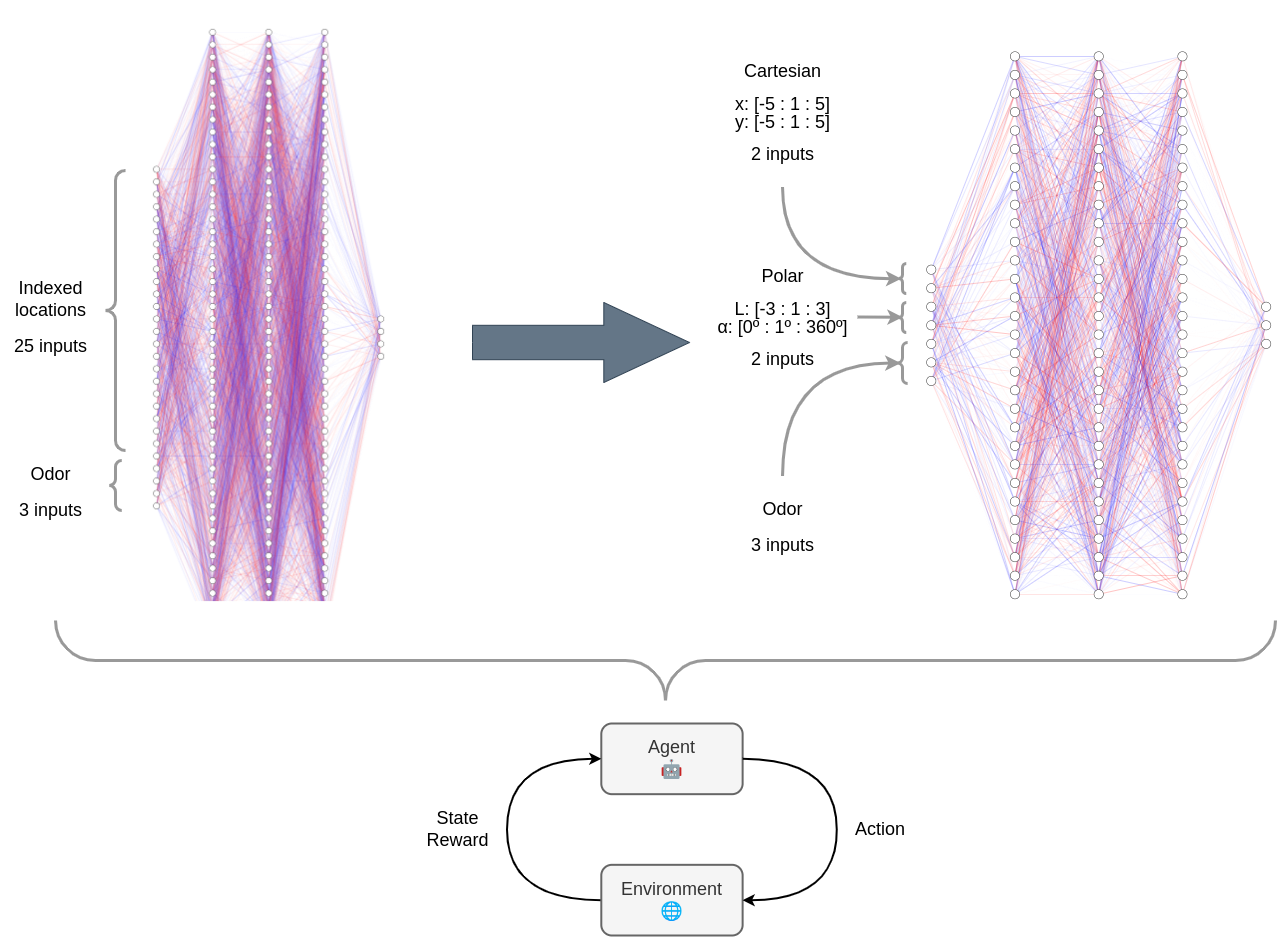
\includegraphics[width=.9\linewidth]{img/nn.drawio.png}
\end{center}
\end{frame}
\begin{frame}[label={sec:orge381525}]{Example episode}
\begin{center}
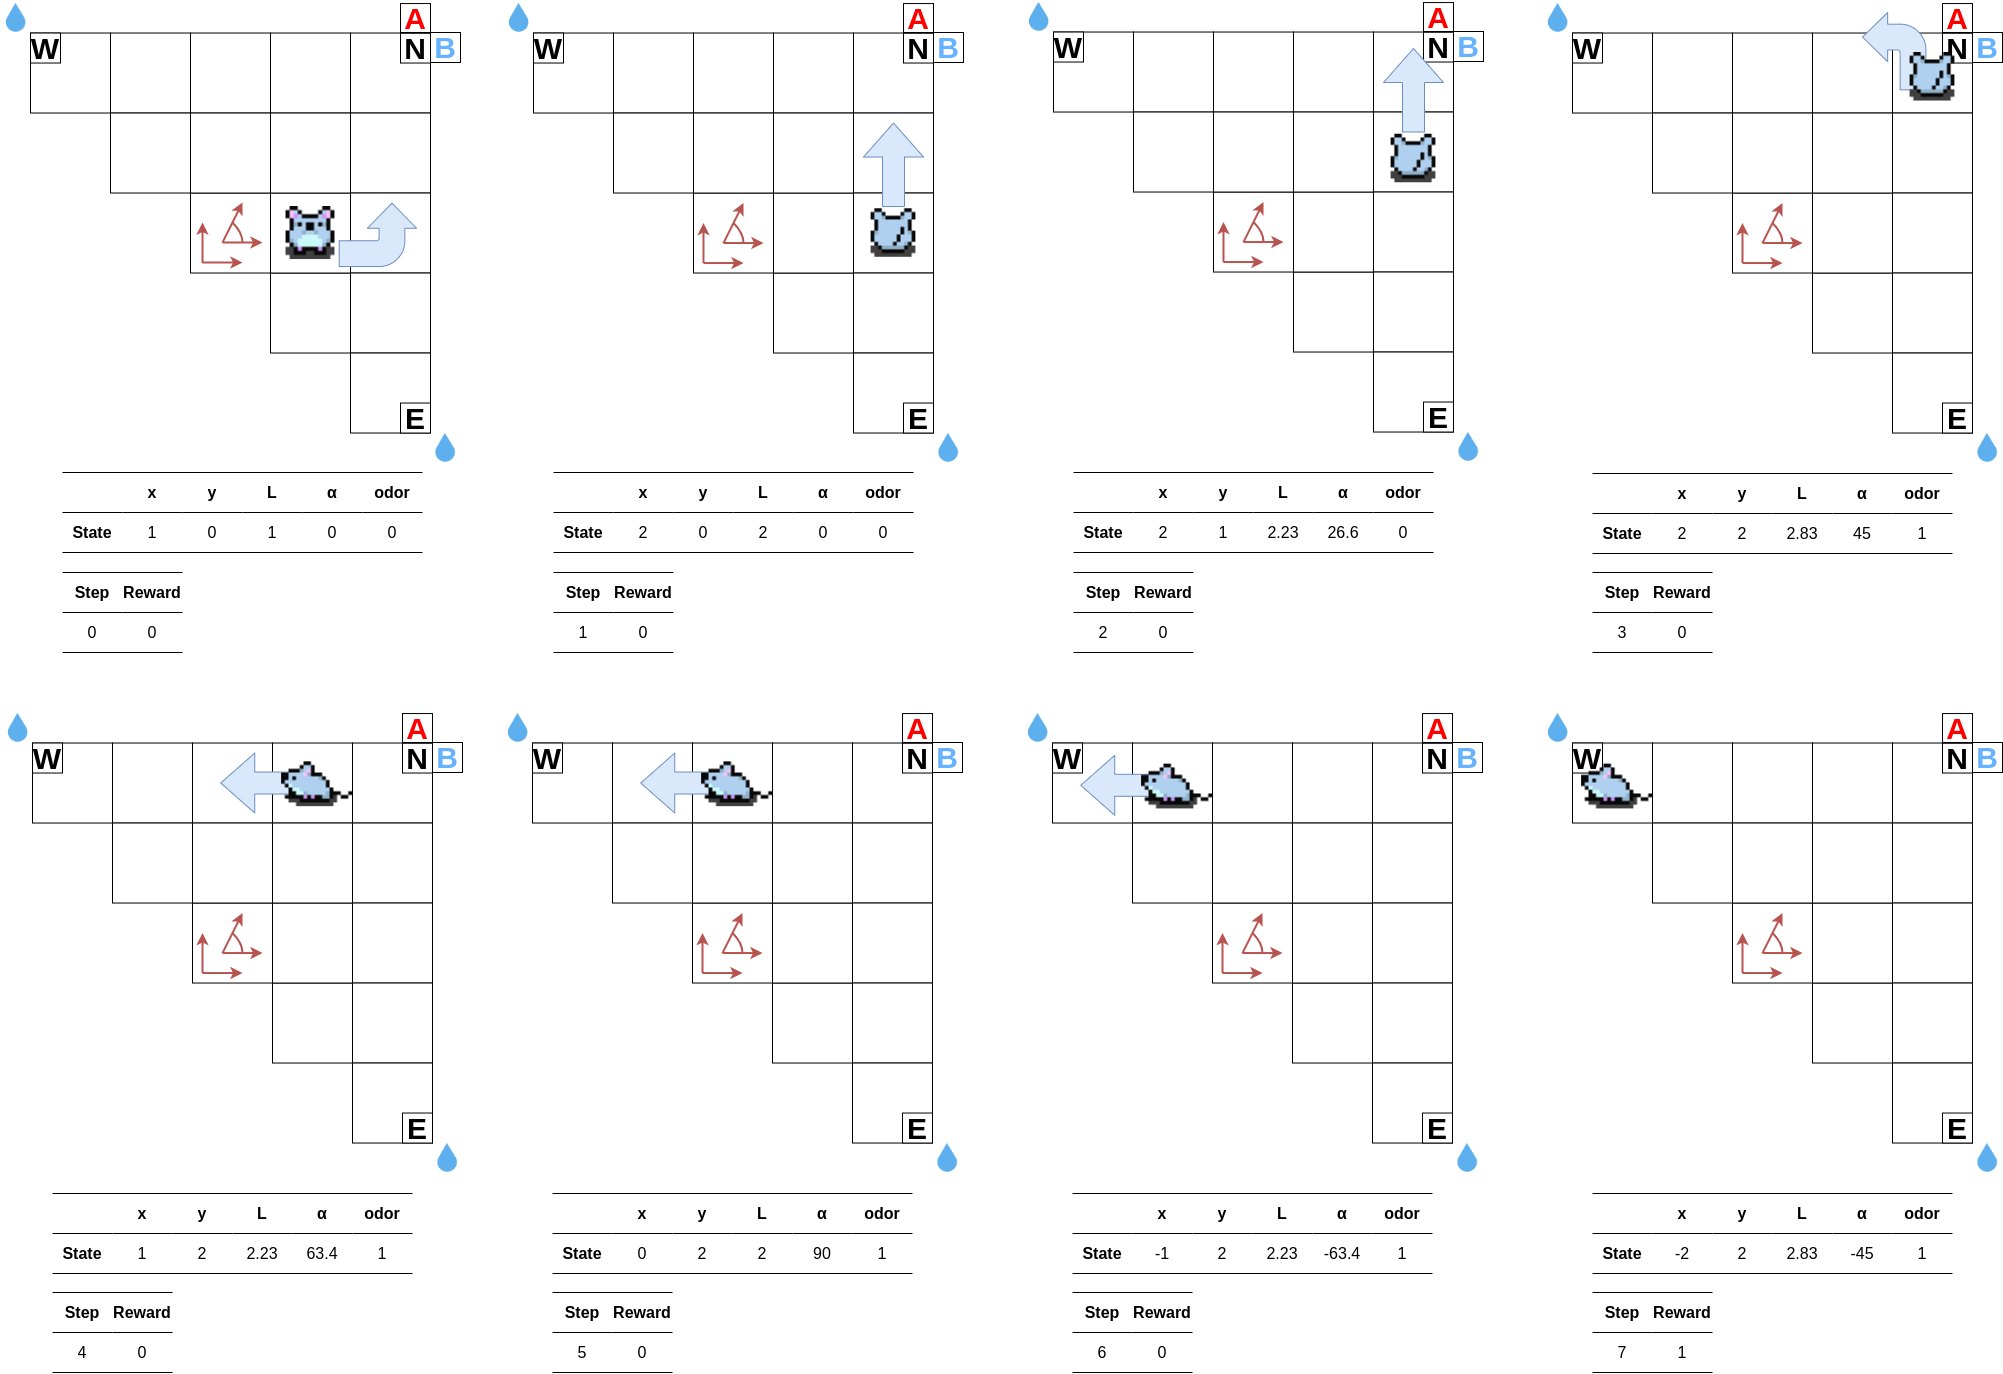
\includegraphics[width=.9\linewidth]{img/env_new-steps.drawio.png}
\end{center}
\end{frame}
\section{Experiments \& expected results \faicon{eyedropper} \faicon{area-chart}}
\label{sec:orgc67c098}
\begin{frame}[<+->][label={sec:org41b93b0}]{1) How training impacts the representations learned?}
\begin{itemize}
\item Feed both coordinates information (Cartesian \& polar) to the input layer (+ merge actions spaces in a common one)
\item Train on left/right task \(\to\) we expect the weights are close to zero on Cartesian representation?
\item Train on east/west task \(\to\) we expect the weights are close to zero on polar representation?
\end{itemize}
\end{frame}
\begin{frame}[label={sec:org31a4945}]{1) How training impacts the representations learned?}
\begin{center}
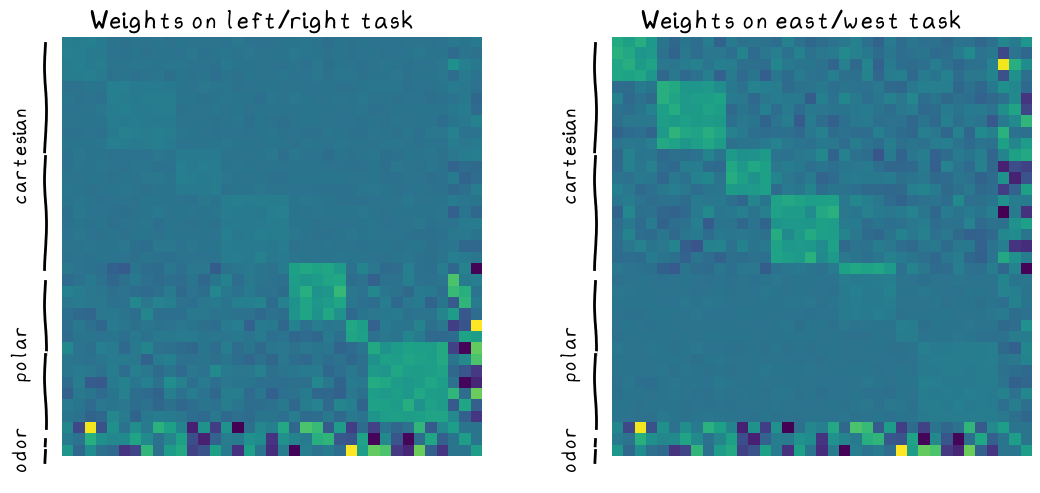
\includegraphics[width=.9\linewidth]{img/exp1-weights-heatmap.png}
\end{center}
\end{frame}
\begin{frame}[<+->][label={sec:orgf6295e5}]{2) Does the network learn a coordinate system?}
\begin{enumerate}
\item After training, move the population of agents in a translated coordinate system
\(\to\) we expect the population of agents to be able to solve the task with zero shot learning
\item Train with both coordinates information (Cartesian \& polar), after training feed incorrect polar angles
\begin{itemize}
\item On the left/right task \(\to\) we expect the population of agents still solves the task consistently
\item On the east/west task \(\to\) we expect the network won't converge to a stable policy (i.e all the agents don't solve the task consistently)
\end{itemize}
\end{enumerate}
\end{frame}
\begin{frame}[label={sec:orgcae1452}]{2) Does the network learn a coordinate system?}
\begin{center}
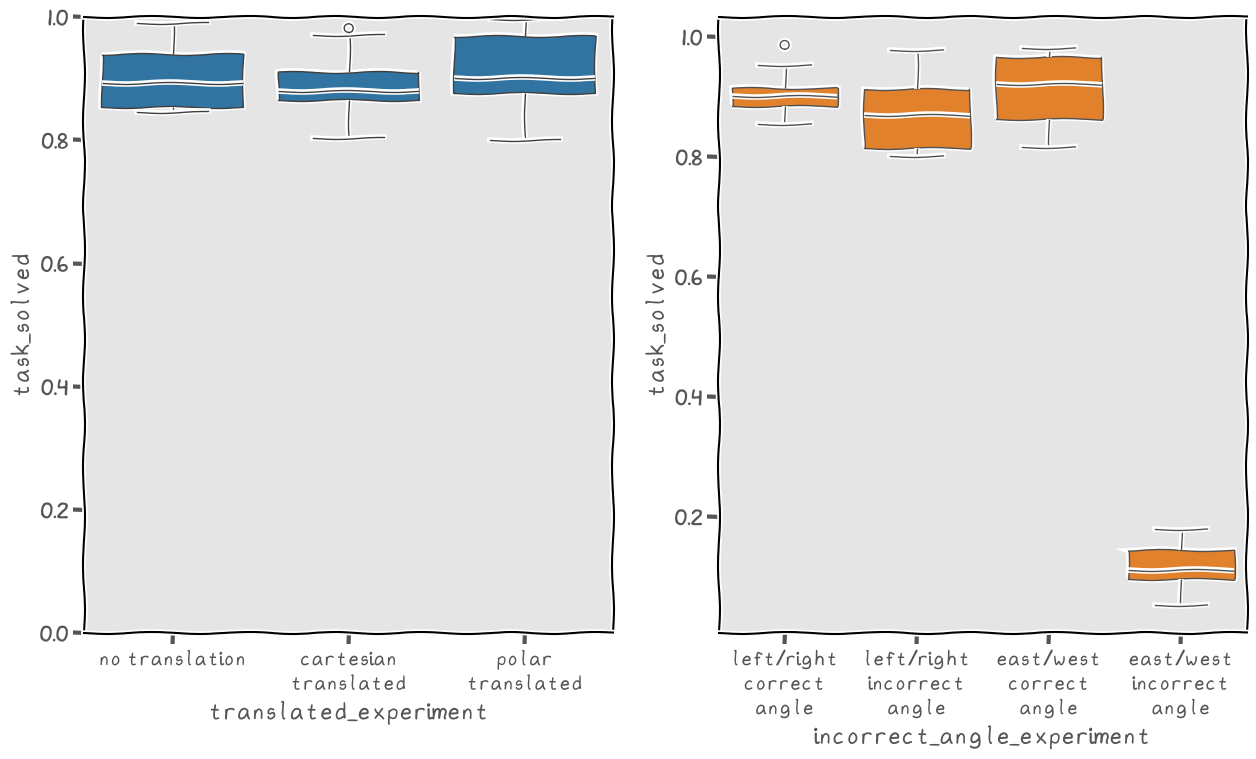
\includegraphics[width=.9\linewidth]{img/exp2-boxplot.png}
\end{center}
\end{frame}
\begin{frame}[label={sec:orgd4bf8ff}]{2) Does the network learn a coordinate system?}
\begin{center}
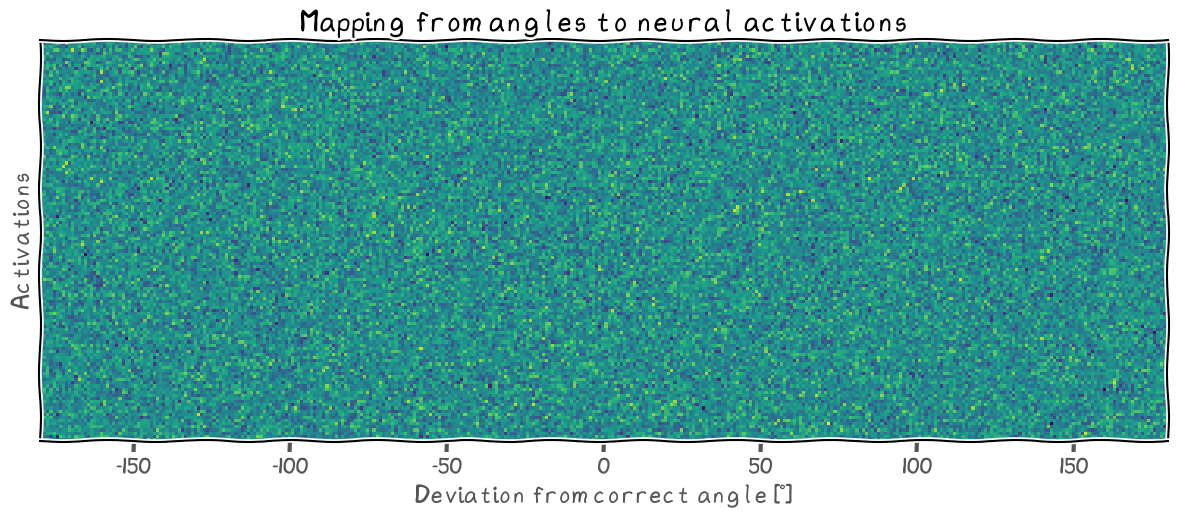
\includegraphics[width=.9\linewidth]{img/angles-to-activations.png}
\end{center}
\end{frame}
\section{Roadmap \faicon{road}}
\label{sec:orgd3cf5fd}
\begin{frame}[label={sec:org817eb6e}]{Experiments table}
\scriptsize
\begin{center}
\begin{tabular}{lrr}
Experiment & Agents & Hours estimation\\
\hline
left/right Cartesian coordinates from center arena & 30 & 6\\
left/right Cartesian coordinates from 3 ports & 30 & 6\\
east/west polar coordinates from center arena & 30 & 6\\
east/west polar coordinates from 3 ports & 30 & 6\\
\hline
No translation & 30 & 6\\
Cartesian translated & 30 & 6\\
Polar translated & 30 & 6\\
left/right correct angle & 30 & 6\\
left/right incorrect angle & 30 & 6\\
east/west correct angle & 30 & 6\\
east/west incorrect angle & 30 & 6\\
\hline
Total & 330 & 66\\
\end{tabular}
\end{center}
\end{frame}
\begin{frame}[<+->][label={sec:orgb70ba54}]{Milestones/how to get there}
\begin{enumerate}
\item Rewrite the environment(s) \faicon{star}\faicon{star}\faicon{star-o}
\begin{enumerate}
\item Code logic for new environment \colorbox{black!15!white}{[$\textasciitilde$1 week]}
\item Check everything works as expected (unit testing) \colorbox{black!15!white}{[$\textasciitilde$1 week]}
\item Bugs? \colorbox{black!15!white}{[$\textasciitilde$1 week]}
\item Baseline training on new environment (convergence, hyperparameter tweaking, etc.) \faicon{star}\faicon{star}\faicon{star}\faicon{warning} \colorbox{black!15!white}{[1 week -- 1 month]}
\end{enumerate}
\item Experiments
\begin{enumerate}
\item Task code \faicon{star}\faicon{star-o}\faicon{star-o} \colorbox{black!15!white}{[$\textasciitilde$1 week]}
\item Training \faicon{star}\faicon{star}\faicon{star-o}\faicon{warning} \colorbox{black!15!white}{[$\textasciitilde$2 week]}
\item Analysis code \faicon{star}\faicon{star}\faicon{star-o} \colorbox{black!15!white}{[$\textasciitilde$2 week]}
\end{enumerate}
\end{enumerate}
\end{frame}
\begin{frame}[label={sec:org9acd4e9}]{Planning}
% \begin{figure}%[htb]
    % \centering
    \begin{adjustbox}{max width=\columnwidth, keepaspectratio}
    \begin{ganttchart}[
        y unit title=1.5em,
        y unit chart=1.3em,
        x unit=0.4em,
        vgrid,
        time slot format=isodate,
        time slot unit=day,
        title/.append style={draw=none, fill=white!20!black},
        title label font=\sffamily\bfseries\color{white},
        title left shift=.05,
        title right shift=-.05,
        title height=1,
        bar/.append style={draw=none, fill=white!50!black},
        bar height=.6,
        bar label font=\normalsize\color{black!50},
        group right shift=0,
        group top shift=.6,
        group height=.2,
        group peaks height=.3,
        bar incomplete/.append style={fill=Maroon},
        link bulge=2,
        calendar week text=W~\currentweek,
        % link tolerance=.1,
        % link/.style={-},
        ]{2024-05-13}{2024-09-15}
        \gantttitlecalendar{year, month=shortname, week=20} \\

        \ganttgroup{New baseline}{2024-05-27}{2024-07-07} \\
        \ganttbar{New environment(s) logic}{2024-05-27}{2024-06-02} \\
        \ganttlinkedbar{Unit testing}{2024-06-03}{2024-06-09} \\
        \ganttlinkedbar{Debugging?}{2024-06-10}{2024-06-16} \\
        \ganttlinkedbar{New baseline training \faicon{warning}}{2024-06-17}{2024-07-07} \\

        \ganttgroup{Experiments}{2024-07-22}{2024-09-08} \\
        \ganttbar{Tasks code}{2024-07-22}{2024-07-28} \\
        \ganttlinkedbar{Training \faicon{warning}}{2024-08-05}{2024-08-25} \\
        \ganttlinkedbar{Analysis}{2024-08-26}{2024-09-08} \\

        \ganttgroup{Misc.}{2024-05-20}{2024-08-04} \\
        \ganttbar{NWB paper}{2024-05-20}{2024-05-26} \\
        \ganttbar{DL+RL summer school}{2024-07-08}{2024-07-17} \\
        \ganttbar{Holidays}{2024-07-29}{2024-08-04} \\
    \end{ganttchart}
    \end{adjustbox}
% \end{figure}
\end{frame}
\begin{frame}[label={sec:org4979371},standout]{~}
Thanks!
\end{frame}
\end{document}
